\documentclass[tikz,border=10pt]{standalone}
\usepackage{tikz}
\usepackage{amsmath}

\begin{document}
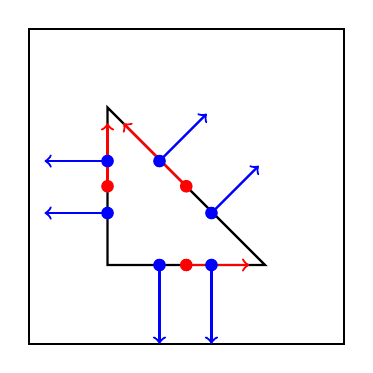
\begin{tikzpicture}[scale=2]

    \coordinate (G0) at (-0.5,-0.5);  
    \coordinate (G1) at (-0.5,1.5);  
    \coordinate (G2) at (1.5,1.5);  
    \coordinate (G3) at (1.5,-0.5);  
    \draw[black, thick] (G0) -- (G1) -- (G2) -- (G3) -- cycle;



    % Define the vertices of the reference triangle
    \coordinate (A) at (0,0);
    \coordinate (B) at (1,0);
    \coordinate (C) at (0,1);
    \coordinate (T1) at (0.5,0);
    \coordinate (T2) at (0,0.5);
    \coordinate (T3) at (0.5,0.5);
    \coordinate (N1) at (0.33,0);
    \coordinate (N2) at (0.66,0);
    \coordinate (N3) at (0.33,0.66);
    \coordinate (N4) at (0.66,0.33);
    \coordinate (N5) at (0,0.33);
    \coordinate (N6) at (0,0.66);




    \draw[black, thick] (A) -- (B) -- (C) -- cycle;

    \draw[->, red, thick] (0.5, 0) -- (0.9, 0);   
    \draw[->, red, thick] (0, 0.5) -- (0, 0.9);   
    \draw[->, red, thick] (0.5, 0.5) -- (0.1,0.9);   
    \draw[->, blue, thick] (0.33, 0.0) -- (0.33,-0.5);   
    \draw[->, blue, thick] (0.66, 0.0) -- (0.66,-0.5);   
    \draw[->, blue, thick] (0, 0.33) -- (-0.4, 0.33);  
    \draw[->, blue, thick] (0, 0.66) -- (-0.4, 0.66);  
    \draw[->, blue, thick] (0.33, 0.66) -- (0.63, 0.96);  
    \draw[->, blue, thick] (0.66, 0.33) -- (0.96, 0.63);  

    \fill[red] (T1) circle (0.04);
    \fill[red] (T2) circle (0.04);
    \fill[red] (T3) circle (0.04);
    \fill[blue] (N1) circle (0.04);
    \fill[blue] (N2) circle (0.04);
    \fill[blue] (N3) circle (0.04);
    \fill[blue] (N4) circle (0.04);
    \fill[blue] (N5) circle (0.04);
    \fill[blue] (N6) circle (0.04);

\end{tikzpicture}
\end{document}



